\documentclass[headings=standardclasses,headings=big,oneside,a4paper,openany,12pt]{scrbook}

\newcommand {\e}[1]{\mathrm{~#1}}
\newcommand {\E}[1]{\times 10^{#1}}
\newcommand {\vars}{$\Delta E$ and $M_{BC}$}
\newcommand {\btbii}{\texttt{B2BII}}
\newcommand {\decaya}{$B \to K K \ell \nu$}
\newcommand {\decayb}{$B^+ \to K^+ K^- \ell^+ \nu$}

%\usepackage{biblatex}
%\bibliography{mybib.bib} 
\usepackage[slovene,english]{babel}% Recommended
\usepackage{csquotes}% Recommended
\usepackage[sorting=none,firstinits=true,backend=bibtex]{biblatex}
\addbibresource{mybib.bib}% Syntax for version >= 1.2

\usepackage{paralist}
\usepackage{caption}
\usepackage{cancel}

\usepackage{longtable}

\setlength{\parskip}{1em}%
\setlength{\parindent}{0cm}

\usepackage{titling}
\usepackage{amsmath,amssymb,amsfonts,nicefrac}
\usepackage{graphicx}
\usepackage{color}
\usepackage{float}
\usepackage{mathtools}
\allowdisplaybreaks
\usepackage[pdftex,colorlinks=true,citecolor=blue,linkcolor=black,urlcolor=blue,bookmarks=true]{hyperref}
\usepackage{dictsym}
\usepackage{braket}
\usepackage{slashed}
\DeclareMathOperator{\arcsinh}{arcsinh}
\usepackage{enumerate}
\usepackage{array}
\setlength{\extrarowheight}{.5ex}

\usepackage{lineno}
\linenumbers

\usepackage{subfigure}

\usepackage{titlesec}
\titlespacing*{\subsubsection}
{0pt}{0pt}{0pt}


\begin{document}
\begin{otherlanguage}{slovene}
\chapter{Povzetek doktorskega dela}
\section{Uvod}
Fizika delcev je eden od stebrov fizike, z mo"cnimi koreninami, ki segajo vse do za"cetka 20. stoletja. Natan"cni eksperimenti in preverljiva teorija so pokazali, da vesolje sestoji iz osnovnih delcev in nosilcev interakcij. Osnovne delce delimo na kvarke ($u$, $d$, $s$, $c$, $b$, $t$) in leptone, ki so nadaljnje razdeljeni na nabite leptone ($e$, $\mu$, $\tau$) in pa nevtrine ($\nu_e$, $\nu_\mu$, $\nu_\tau$). Nosilci treh (od "stirih) osnovnih interakcij, s katerimi se ukvarjamo na tem podro"cju, so fotoni ($\gamma$) za elektromagnetno, gluoni ($g$) za mo"cno in nabiti- ($W^\pm$) ter nevtralni ($Z^0$) bozoni za "sibko interakcijo. Vsi delci in njihovi zrcalni partnerji, antidelci (ozna"ceni z $~\bar {}~$), imajo maso, ki jim jo dolo"ca Higgsov bozon ($H$). Vse delce ter interakcije med njimi opisuje Standardni model, ki je osrednja teorije fizike visokih energij. Kvarke lahko zdru"zujemo v kombinacije oblike $q_1 q_2 q_3$ (hadroni) ali pa $q_1 \bar{q}_2$ (mezoni), med katere sodijo tudi protoni in nevtroni, ki jih opazimo v naravi. Poleg omenjenih dolgo-"zive"cih delcev pa obstajajo tudi te"zji, manj stabilni delci, ki preko zgoraj na"stetih interakcij razpadejo v la"zje, stabilnej"se. Raziskovanje tak"snih procesov s pomo"cjo pospe"sevalnikov in trkalnikov nam omogo"ca spoznavanje zakonov vesolja danes pa vse do njegovega za"cetka.

Osrednji del doktorske disertacije predstavljajo meritve razpadov mezonov $B$, delcev, ki so sestavljeni iz te"zkega kvarka $b$ in enega od lahkih kvarkov $u$ ali $d$. Ena bolj presenetljivih lastnosti vesolja je kr"sitev simetrije $CP$, t.j. kombinacije simetrij konjugacije naboja ($C$) in prostorske inverzije ($P$). Simetrija $CP$ nakazuje, da so fizikalni procesi delcev in zrcalni procesi antidelcev enaki, kar pa danes vemo, da ne dr"zi v celoti in poznamo procese, ki to simetrijo kr"sijo. Kr"sitev simetrije $CP$ je tesno povezana s "sibko interakcijo, to pa predstavlja na"so motivacijo za "studijo mezonov $B$, saj "sibki razpadi predstavljajo ve"cji del vseh razpadov mezonov $B$.

Edinstvena lastnost "sibke interakcije je, da lahko spreminja tip oziroma t.i. okus kvarkov, medtem ko ga ostale interakcije ohranjajo. Tak"sni procesi so opisani s prehodno matriko CKM (Cabibbo-Kobayashi-Maskawa) \cite{cabibbo1963unitary,kobayashi1973cp}
\begin{equation}
V_{CKM} = \begin{bmatrix}
    V_{ud} & V_{us} & V_{ub}\\
	V_{cd} & V_{cs} & V_{cb}\\
	V_{td} & V_{ts} & V_{tb}
\end{bmatrix}.
\end{equation}
Unitarnost matrike CKM nam omogo"ca, da iz nje izlu"s"cimo matemati"cne identitete, od katerih je ena pomembnej"sih
\begin{equation}
V_{ud}V_{ub}^* + V_{cd}V_{cb}^* + V_{td}V_{tb}^* = 0,
\end{equation}
poznana pod imenom unitarni trikotnik, saj predstavlja zaklju"cen vektor treh to"ck v kompleksni ravnini, kot prikazuje Slika \ref{fig:ut_si}. Parametri matrike CKM niso dolo"cljivi s strani teorije, temve"c jih moramo dolo"citi z eksperimentalnimi meritvami tako, da najdemo procese, ki so tesno povezani s stranicami in koti unitarnega trikotnika. Na tak na"cin lahko preverimo, "ce je oblika trikotnika konsistentna, kar predstavlja dober test Standardnega modela, oziroma "ce so potencialno prisotni kak"sni novi procesi, ki jih "se ne poznamo, in jih kolektivno imenujemo "nova fizika". Dodatna motivacija za "studijo mezonov $B$ je ta, da velik dele"z njihovih razpadov predstavlja koristne procese za meritev unitarnega trikotnika.
\begin{figure}[H]
\centering
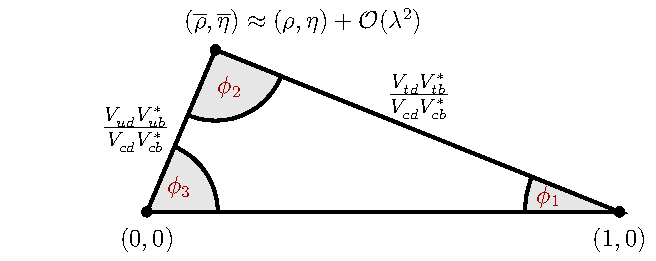
\includegraphics[scale=1]{texfig/UT_Triangle}
\caption{Unitarni trikotnik s parametri $\lambda,~\eta,~\rho$ and $A$ (slednji ni prikazan), ki predstavljajo proste parametre matrike CKM.} %TODO: Wolf. param. 
\label{fig:ut_si}
\end{figure}

Procesi, ki jih "studiramo v tej analizi, so tesno povezani z elementom $V_{ub}$ matrike CKM, saj le-ta opisuje prehode kvarkov $b \to c$. Od vseh elementov, je absolutna vrednost tega elementa najmanj"sa, relativna napaka pa najve"cja, zato meritve iz tega podro"cja potencialno omogo"cajo najve"c izbolj"save. Tak"sni prehodi kvarkov so prisotni v nečarobnih (t.j. brez kvarkov $c$) semi-leptonskih razpadih mezonov $B$ oblike 
\begin{equation}
B^+ \to X_u^0 \ell^+ \nu_\ell,
\end{equation}
kjer $X_u^0$ predstavlja ne"carnobne mezone, $\ell$ pa je eden od nabitih leptonov. Frekvenco razpadov, ki je tesno povezana z elementom $V_{ub}$, opi"semo z ena"cbo
\begin{equation}
\mathrm{d} \Gamma \propto G_F^2 \vert V_{ub} \vert ^2 \vert L^\mu \langle X_u \vert \bar u \gamma_u \frac{1}{2} (1-\gamma_5) b \vert B \rangle \vert ^2,
\end{equation}
kjer $G_F$ predstavlja Fermijevo konstanto, $L^\mu$ leptonski tok, izraz v Diracovih oklepajih pa hadronski tok. V tak"snih prehodih $\vert V_{ub} \vert ^2$ predstavlja verjetnost za prehod $b \to u$.

Meritev elementa $V_{ub}$ je mo"zna na ekskluziven in inkluziven na"cin, kjer pri prvi metodi opravljamo meritve v specifi"cno definirana kon"cna stanja, kot na primer $B \to \pi \ell \nu$, pri drugi metodi pa opravljamo meritev s kupno kon"cno stanje oblike $B \to X_u \ell \nu$. Obe metodi potekata preko razli"cnih pristopov in se soo"cata z razli"cnimi tezavami, kar pomeni, da sta oba kon"cna rezultata nekorelirana. Rezultata obeh meritev imata tudi zelo podobno natan"cnost, medtem ko se srednja vrednost le deloma ujema. Rezultata se razlikujeta s signifikanco $3\sigma$, kar predstavlja ve"cjo te"zavo znotraj podro"cja. Trenutni svetovni povpre"cji \cite{Amhis:2016xyh} ekskluzivne (iz razpadov $B^0 \to \pi^- \ell^+ \nu$) in inkluzivne meritve (GGOU kolaboracija \cite{Gambino:2007rp}) sta
\begin{align}
&\vert V_{ub} \vert_{\mathrm{e.}} = \left(3.65 \pm 0.09 \pm 0.11\right)\E{-3},\\
&\vert V_{ub} \vert_{\mathrm{i.}}^{\mathrm{GGOU}} = \left(4.52 \pm 0.15~{}^{+0.11}_{-0.14}\right)\E{-3},
\end{align}
kjer prva in druga napaka predstavljata eksperimentalno in teoretsko napako. Rezultati inkluzivnih meritev so praviloma ve"cji kot rezultati ekskluzivnih. Razlogov za neujemanje je lahko ve"c, od nepoznanih napak pri eksperimentu ali teoriji, do prispevkov nove fizike.

V tej analizi se osredoto"camo na enega od mo"znih razlogov za zgoraj omenjeno neujemanje, konkretneje za razpad \decayb, ki je strukturno precej podoben razpadu $B \to \pi \ell \nu$ za razliko produkcije para kvarkov $s \bar s$ ki se potem hadronizira v nove delce, kot prikazuje Slika \ref{feynman}. V inkluzivnih meritvah ne"carobnih semi-leptonskih razpadov mezonov $B$ se standardno uporablja $K$-veto, t.j. selekcija, kjer zahtevamo, da v kon"cnem stanju nimamo mezonov $K$ (sestava $q \bar s,~q \in [u,d]$), poznanih tudi pod imenom kaoni. Kaoni v kon"cnem stanju nakazujejo na pogost prehod kvarkov $b \to c \to s$, ki pa jih ho"cemo v analizah prehodov $b \to u$ zatreti. V primeru na"se analize imamo v kon"cnem stanju 2 kaona s prehodom $b \to u$, kar pomeni, da tak"sni razpadi niso upo"stevani v inkluzivnih meritvah, "ceprav bi morali biti. Cilj "studije je dolo"citi pogostost razpadov \decayb~s prehodom $b\to u$ in s tem oceniti, kak"sen potencialen efekt ima lahko neupo"stevanje teh razpadov na inkluzivno meritev elementa $V_{ub}$. V nadaljevanju bo razpad \decayb~zaradi enostavnosti zapisan kot \decaya.
\begin{figure}[H]
\centering
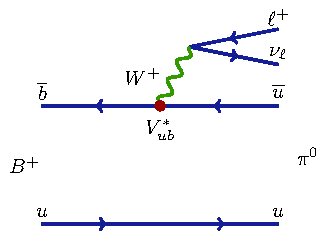
\includegraphics{texfig/B2pilnu}
\hspace{1cm}
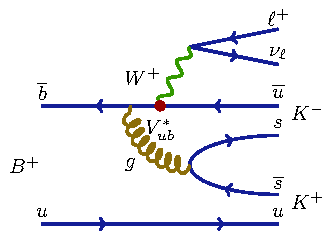
\includegraphics{texfig/B2KKlnu}
\caption{Feynmanovi diagrami za razpada $B^+ \to \pi^0 \ell^+ \nu_\ell$ (levo) in $B^+ \to K^- K^+ \ell^+ \nu_\ell$ (desno).}
\label{feynman}
\end{figure}

\section{Experimentalna postavitev}

Podatki, uporabljeni v tej analizi, so bili ustvarjeni pri trkih elektronov $e^-$ in pozitronov $e^+$ v pospeševalniku KEKB in zajeti z detektorjem Belle. Eksperiment je trajal od leta 1999 do 2010 pod okriljem znanstvene organizacije KEK v mestu Tsukuba na Japonskem. Trki delcev so se dogajali pri energiji, ki je ustrezala masi resonance $\Upsilon(4S)$, (sestava $b \bar b$). V tem delu disertacije sta opisana pospeševalnik in detektor, podrobnejši opis pa se nahaja v literaturah \cite{doi:10.1093/ptep/pts102} in \cite{ABASHIAN2002117}.

\subsection{Trkalnik KEKB}

KEKB je asimetričen trkalnik delcev $e^+e^-$, ki potujejo po obročih s premerom $3\e{km}$ v gručah. V središču detektorja gruči elektronov z energijo $8\e{GeV}$ in pozitronov z energijo $3.5\e{GeV}$ trčita pod kotom $22\e{mrad}$. Skupna invariantna masa trka ustreza masi resonance $\Upsilon(4S)$ 
\begin{equation}
E_{CM} = 2\sqrt{E_{e^+}E_{e^-}} = m_{\Upsilon(4S)}c^2 \approx 10.58\e{GeV}.
\end{equation}
Delež mezonov $\Upsilon(4S)$ razpade preko zelo čistega kanala v dva praktično mirujoča mezona $B$, kar tej in v podobnih analizah pogosto izkoriščamo, saj je začetno stanje dobro poznano.

Trkalnik je v času obratovanja zajel količino podatkov, ki ustreza integrirani luminoznosti $1041\e{fb^{-1}}$, od katere okoli $711\e{fb^{-1}}$ predstavlja podatke, zajete pri energiji $10.58\e{GeV}$, t.j. masi resonance $\Upsilon(4S)$. Slednja vrednost integrirane luminoznosti ustreza številu $771\E{6}$ parov $B \bar B$ mezonov.

\subsection{Detektor Belle}
Detektor Belle je magnetni masni spektrometer, ki pokriva ve"cji del prostorskega kota. Njegov namen je, da detektira delce, ki se gibljejo v magnetnem polju $1.5\e{T}$ in so potomci trkov $e^+e^-$. Cilj je dolo"citi energijo in gibalno koli"cino delcev, kar dose"zemo preko detektorskih podsistemov, ki so okoli interacijske to"cke postavljeni v plasteh. Detektor pokriva polarni kot med $17^\circ \leq \theta \leq 150^\circ$, med tem ko je azimutni kot pokrit v celoti, kar skupaj predstavlja $92\%$ pokritost polnega prostorskega kota.
\subsubsection{Silikonski  detektor verteksov}
Silikonski detektor verteksov je postavljen najbli|zje interakcijski to"cki. Sestavljen je iz dvostranskih silikonskih detektorjev, ki podajajo 2D informacijo o prehodih nabitih delcev z natan"cnostjo okoli $100\e{\mu m}$. To nam omogo"ca dolo"citev to"ck razpada (verteksov) kratko-"zivecih delcev.

\subsubsection{Osrednja potovalna komora}
Osrednja potovalna komora je sestavljena iz mnogo "zic, napeljanih skozi me"sanico plina.  Komora tako meri sledi nabitih delcev, ki potujejo skozi magnetno polje v detektorju. Preko sledi lahko dolo"cimo informacijo o gibalni koli"cini delca, hkrati pa v obmo"cju gibalne koli"cine pod $0.8\e{GeV}/c$ slu"zi tudi za njihovo identifikacijo.

\subsubsection{Merilec "casa preleta}
Merilec "casa preleta meri "casovno razliko od trka pa do preleta delca skozi enega od scintilatorjev tega podsistema. Namen je identifikacija delcev v obmo"cju gibalnih koli"cin $0.8\e{GeV}/c < p < 1.2\e{GeV}/c$, "se posebej kaonov $K^\pm$ in pionov $\pi^\pm$. Pri isti gibalni koli"cini zaradi razli"cnih mas delcev dobimo razli"cne case preleta, kar lahko uporabimo za dolo"citev njihove mase. "Casovna resolucijo tega podsistema je bolj"sa kot ali enaka $100\e{ps}$.

\subsubsection{Pragovni "stevec sevanja "Cerenkova}
TOF is not capable of performing good PID above $1.2\e{GeV}/c$ momentum, since $\beta$ is almost equal to 1. For higher momenta in the region $1.0\e{GeV}/c < 4.0\e{GeV}/c$, the ACC is introduced. It is a threshold-type Cherenkov counter which utilizes the fact that particles emit Cherenkov light if the particle speed is greater than the speed of light in the passing medium. ACC is introduced in the barrel region with 960 separate modules, covering a polar angle of $34^\circ < \theta < 127^\circ$ and 228 modules in the forward end-cap region, with the polar angle coverage of $17^\circ < \theta < 34^\circ$. Each ACC module consists of an aluminum encased block of silica aerogel and one or two fine-mesh PMTs encased on each block to detect Cherenkov light pulses. Due to the polar angle dependence of the particle momentum, 6 different refractive indices are chosen for the aerogel material, ranging from $1.010$ up to $1.030$ and are controlled within $3\%$ precision. The layout of the ACC is shown in Figure \ref{fig:ACC_layout}.
\begin{figure}[H]
	\centering
	\captionsetup{width=0.8\linewidth}
	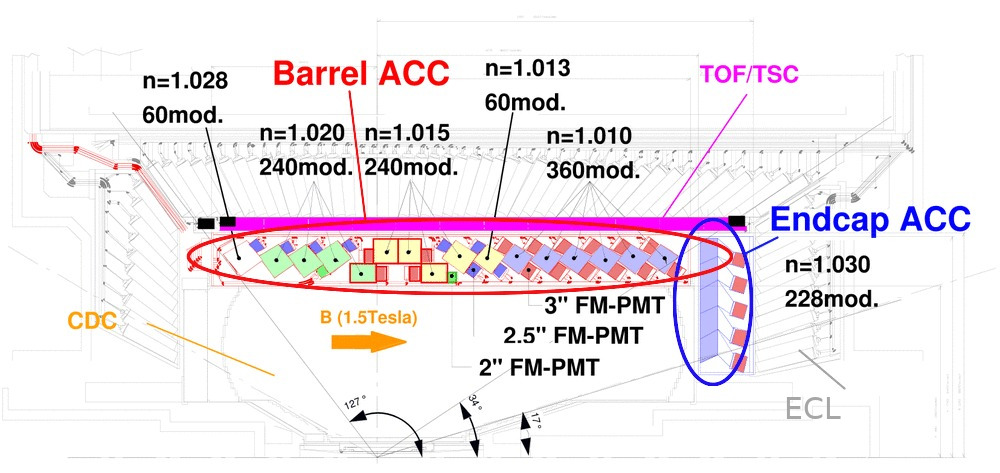
\includegraphics[width=\linewidth]{fig/setup/ACC_layout}
	\caption{Cross-sectional view of the CDC (inner most), ACC and TOF (outer most) detectors \cite{ABASHIAN2002117}.}
	\label{fig:ACC_layout}
\end{figure}
The threshold velocity $\beta$ of a given particle for Cherenkov radiation is
\begin{equation}
\beta \leq \frac{1}{n},
\end{equation}
where $n$ is the refractive index of the medium. The refractive indices in the ACC are such that, due to different masses, pions will emit Cherenkov light and kaons will not, due to different masses of the particles. Using the PID of ACC, along with other sub-system PID info, the electron identification efficiency in the momentum range above $1\e{GeV}/c$ is equal to or above $90\%$ while the pion fake rate, the probability of wrongly identifying pions as electrons, to be around $0.2$ - $0.3\%$. Similarly for kaons, kaon ID efficiency is equal to $80\%$ for most of the momentum region up to $4\e{GeV}/c$, while pion fake rate remains below $10\%$. Figure \ref{fig:ACC_eff} shows the electron and kaon efficiencies and the corresponding pion fake rates as a function of particle momenta.

\begin{figure}[H]
	\centering
	\captionsetup{width=0.8\linewidth}
	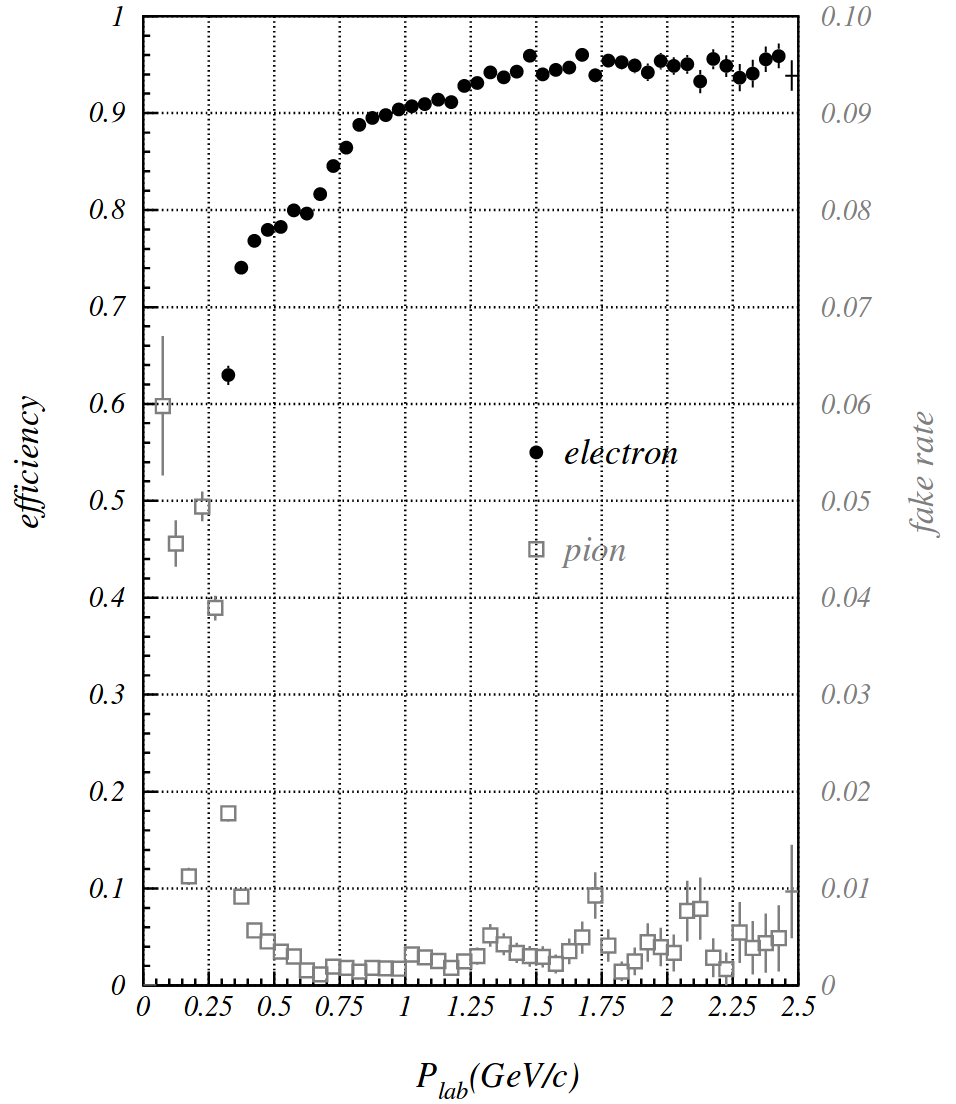
\includegraphics[width=0.48\linewidth]{fig/setup/ACC_eff1}
	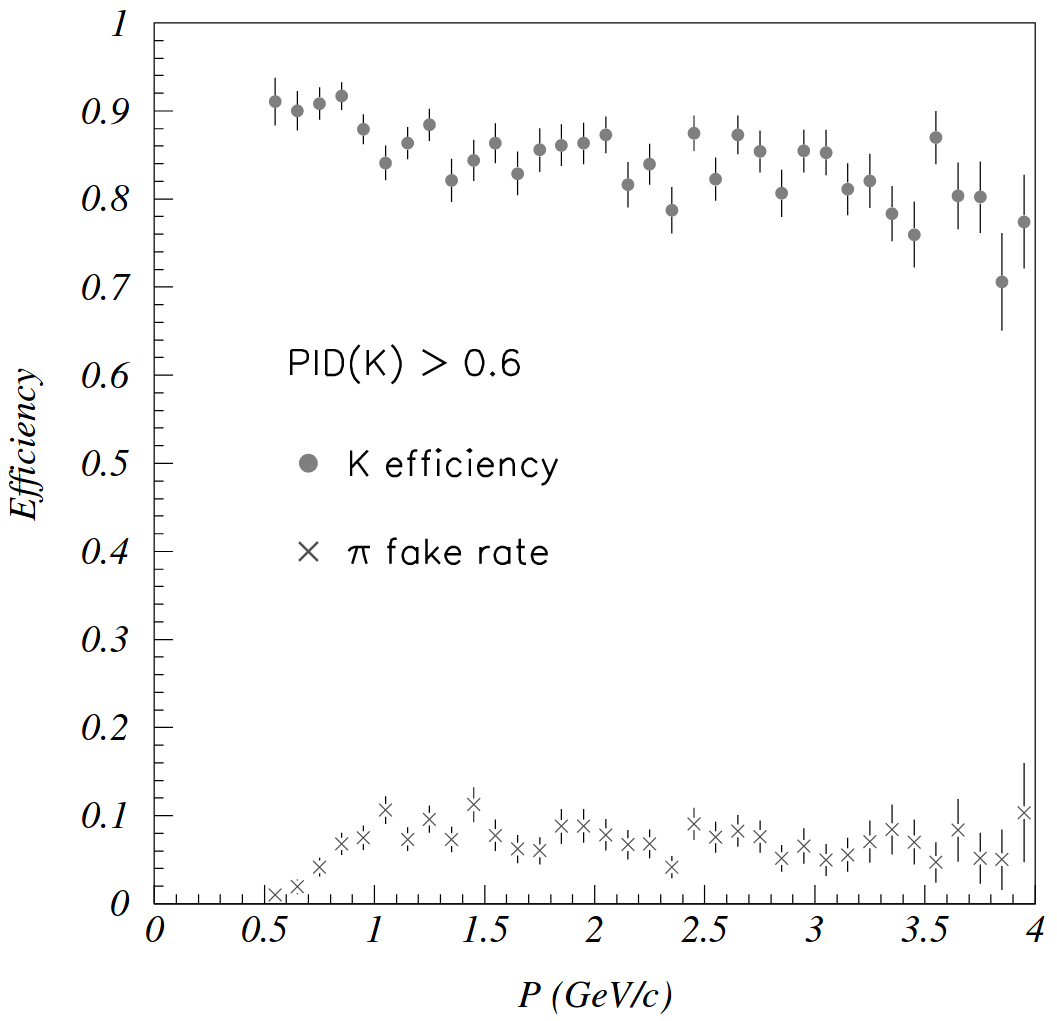
\includegraphics[width=0.48\linewidth,trim = 0cm -4cm 0cm 0cm]{fig/setup/ACC_eff2}
	\caption{Electron identification efficiency and fake rate for charged pions (left) and similarly for kaons (right). Note the different scales for the electron efficiency and fake rate in the former case \cite{ABASHIAN2002117}.}
	\label{fig:ACC_eff}
\end{figure}


\subsubsection{Electromagnetic Calorimeter}
Measurement of position and energy deposit of particles is performed in the ECL, especially for electrons and photons, where the latter are not measured by any of the subsystems described so far. It also provides complimentary particle identifications for electrons versus pions. The calorimeter consists of a highly segmented array of thallium-doped caesium iodide (CsI(Tl)) in the form of tower-shaped crystals, each pointing towards the IP. Each crystal is about $30\e{cm}$ long with a width from $44.5\e{mm}$ to $65\e{mm}$ in the barrel, and from $44.5\e{mm}$ to $82\e{mm}$ in the end-caps. Out of a total of 8736 crystals with a total mass of about $43\e{tons}$, 6624 of them are positioned in the barrel region and 1152 (960) in the forward (backward) end-caps. The inner radius of the barrel section is about $1.25\e{m}$, while the end-caps are positioned at $-1.0\e{m}$ and $2.0\e{m}$ from the IP in direction of the $z$ axis. The polar angle coverage of the barrel region is $32.2^\circ < \theta < 128.7^\circ$, and for the end-caps $12.4^\circ < \theta < 31.4^\circ$ and $130.7^\circ < \theta < 155.1^\circ$. Figure \ref{fig:ECL_layout} shows the layout of the barrel and end-caps ECL. 
\begin{figure}[H]
	\centering
	\captionsetup{width=0.8\linewidth}
   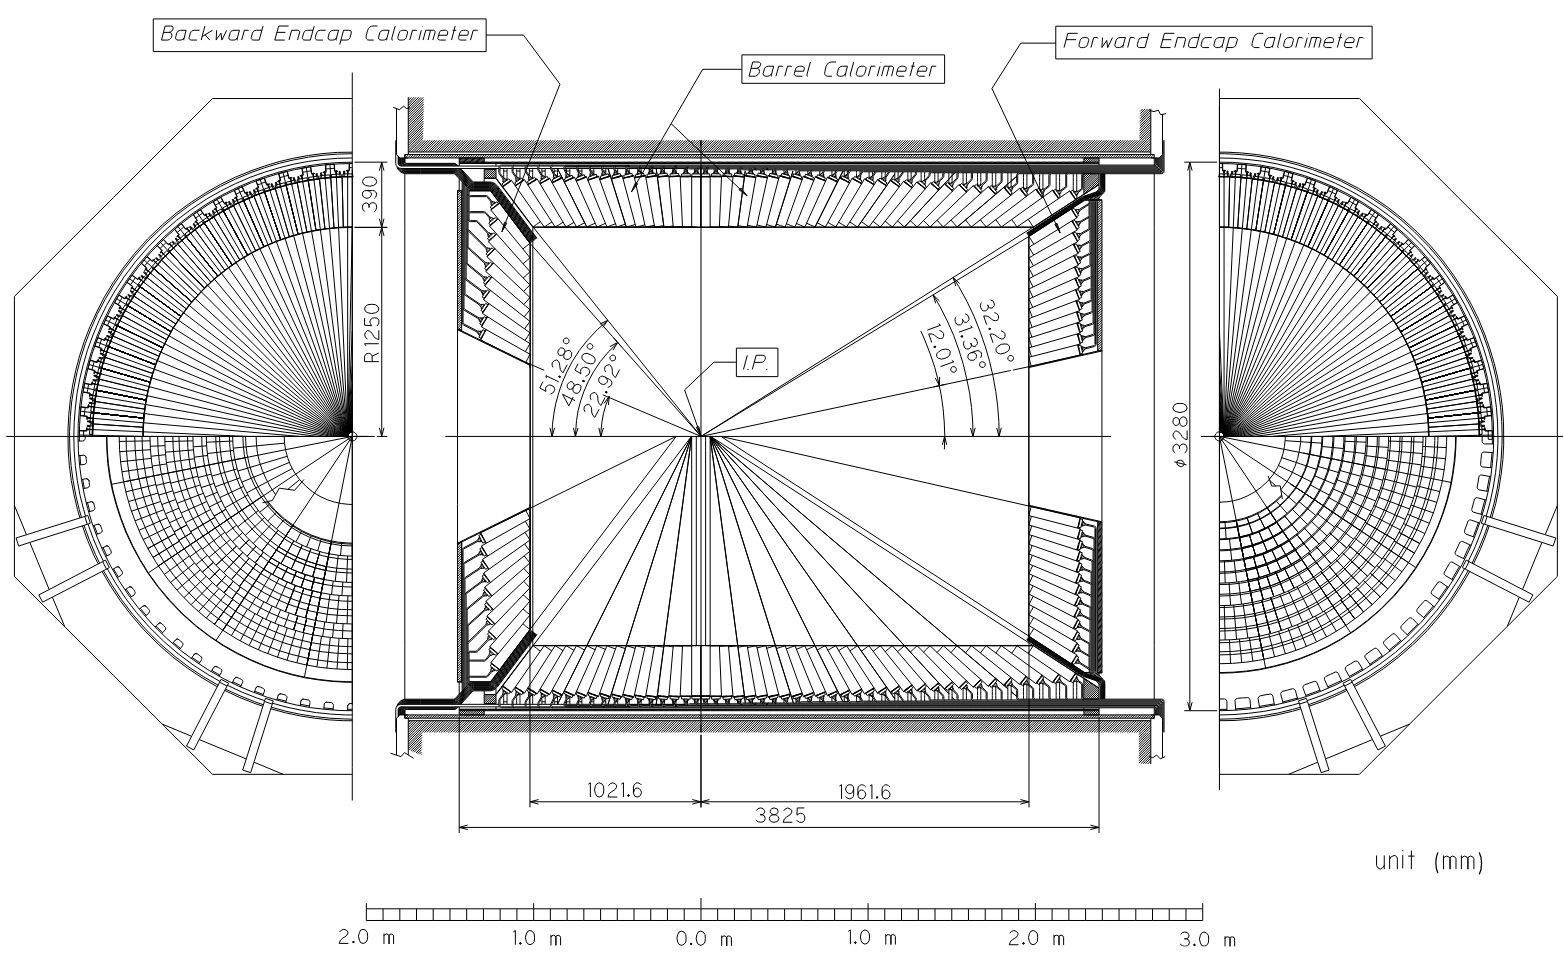
\includegraphics[width=\linewidth]{fig/setup/ECL_layout}
	\caption{Overall configuration of the ECL \cite{ABASHIAN2002117}.}
	\label{fig:ECL_layout}
\end{figure}
When an electron or a photon hits a crystal, it produces an electromagnetic shower, a result of the bremsstrahlung and pair-production effects. Heavier charged particles do not interact in the same way and deposit only a small amount of energy by ionization effects. The information from the ECL, compared with momentum measurements provided by the CDC, enables the identification of electrons. The distribution of the deposited energy for different particles is shown in Figure \ref{fig:ECL_deposit}. The probability of misidentifying an electron as a pion is approximately $5\%$ for momenta less than $1\e{GeV}/c$, and less than $1\%$ for momenta above $2\e{GeV}/c$.

\begin{figure}[H]
	\centering
	\captionsetup{width=0.8\linewidth}
	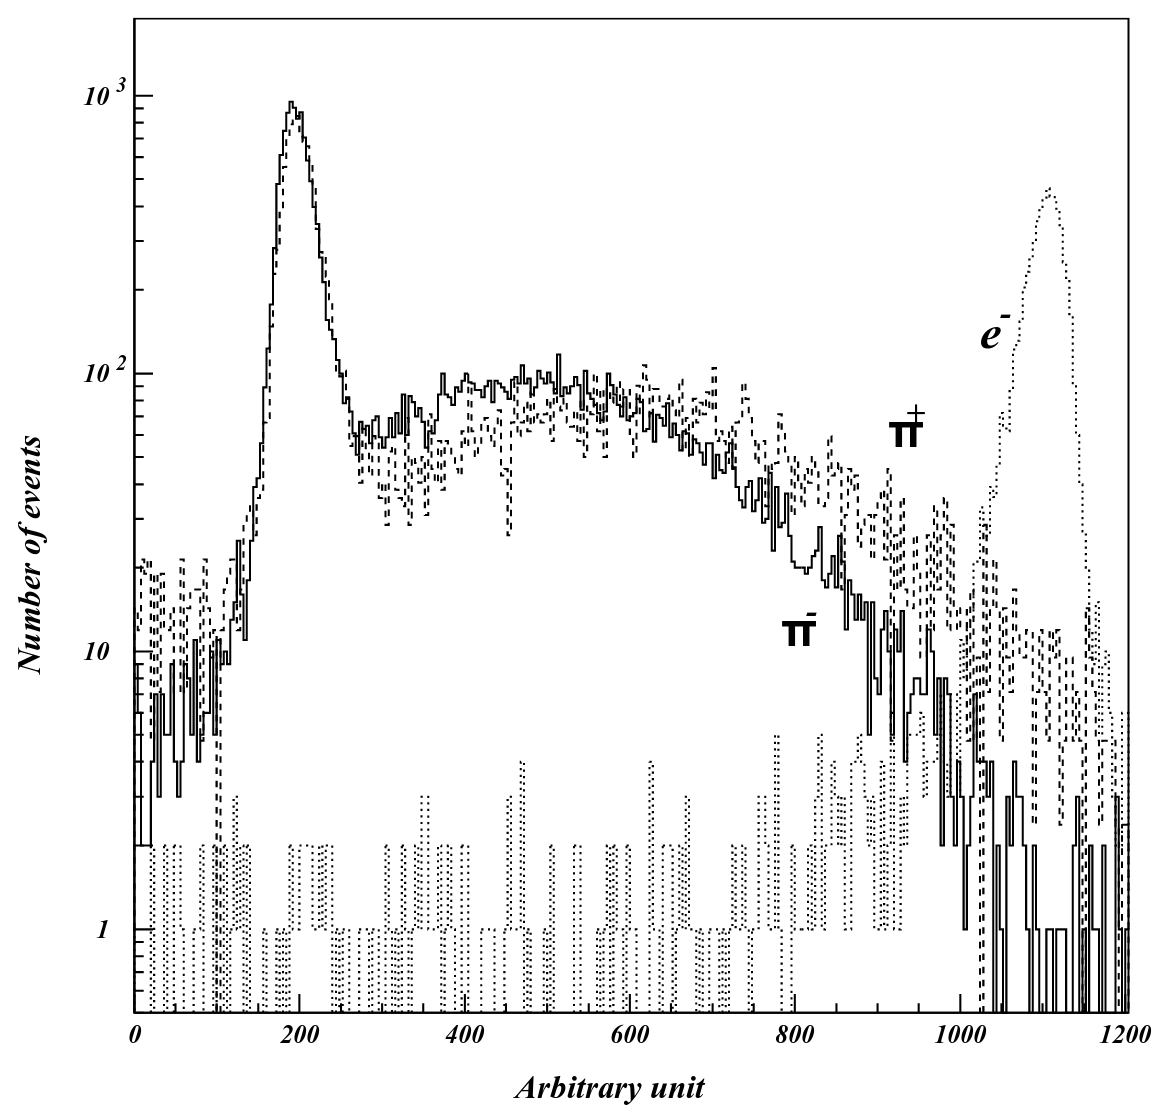
\includegraphics[width=0.6\linewidth]{fig/setup/ECL_deposit}
	\caption{Distribution of the energy deposit by electrons and charged pions at $1\e{GeV}/c$ momentum \cite{ABASHIAN2002117}.}
	\label{fig:ECL_deposit}
\end{figure}

For ECL calibration, $e^+e^- \to e^+e^-$ and $e^+e^- \to \gamma\gamma$ events were used. The average energy resolution was achieved to be $1.7\%$ for the barrel ECL, and $1.74\%$ and $2.85\%$ for the forward and backward ECL, respectively, as shown in Figure \ref{fig:ECL_resolution}. These value are in good agreement with Monte Carlo predictions. Worse energy resolution in backward end-cap is due to the lower photon energy, which results in larger effects of passive material in front of the calorimeter \cite{haba2004letter}. The energy resolution as a function of energy can be obtained via the following relation
\begin{equation}
\frac{\sigma_E}{E} = \frac{0.0066\%}{\left(E/1\e{GeV}\right)}\oplus\frac{1.53\%}{\left( E/1\e{GeV}\right)^{1/4}}\oplus 1.18\%,
\end{equation}
while the resolution of the position measurement is
\begin{equation}
\sigma_{pos} = 0.27\e{mm}+\frac{3.4\e{mm}}{\left( E/1\e{GeV}\right)^{1/2}} + \frac{1.8\e{mm}}{\left( E/1\e{GeV}\right)^{1/4}}.
\end{equation}

\begin{figure}[H]
	\centering
	\captionsetup{width=0.8\linewidth}
	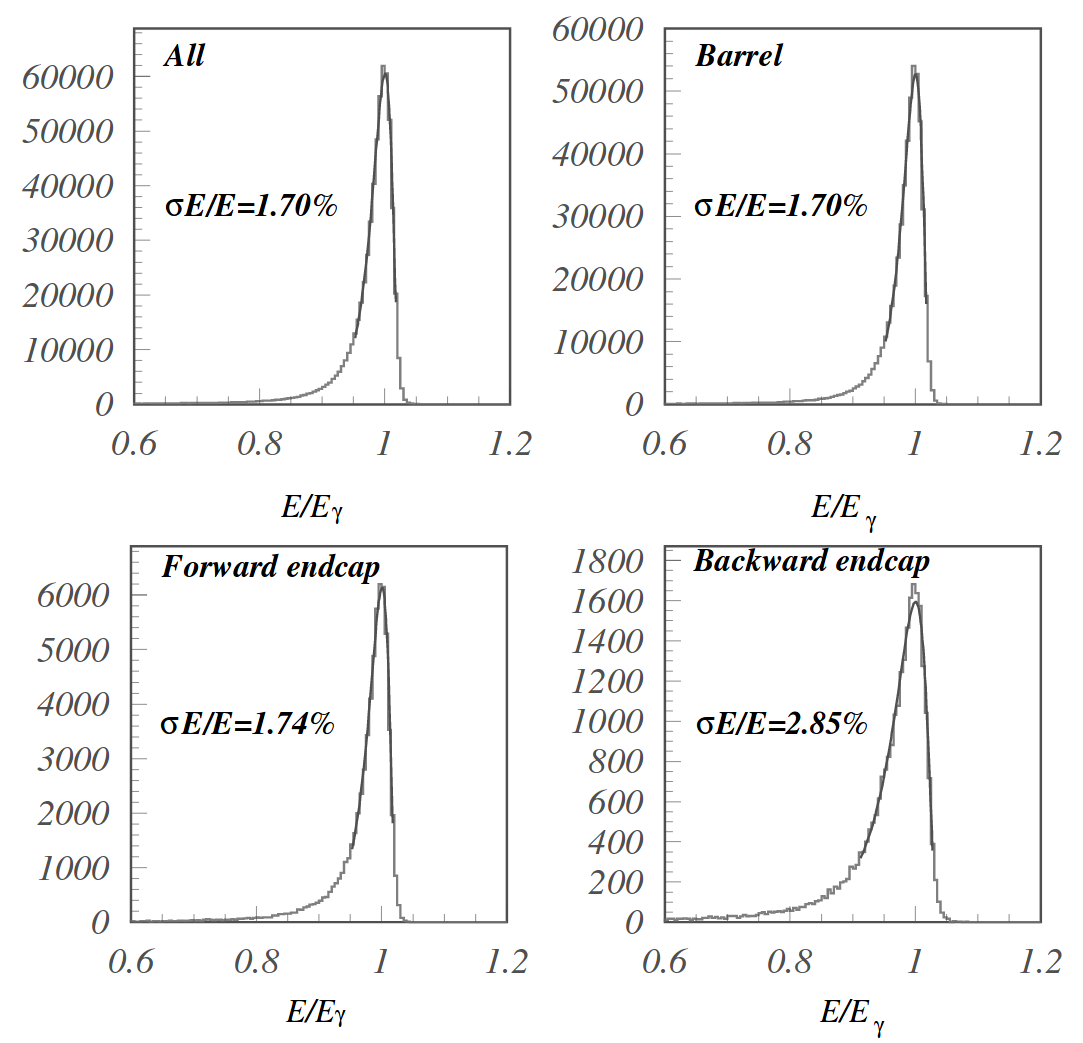
\includegraphics[width=0.8\linewidth]{fig/setup/ECL_resolution}
	\caption{Reconstructed energy distribution for $e^+e^- \to \gamma\gamma$ events for overall, barrel, forward and backward end-cap calorimeters \cite{ABASHIAN2002117}.}
	\label{fig:ECL_resolution}
\end{figure}

\subsubsection{$K_L^0/\mu$ Detector}
The KLM detector is used for detection of high-penetration particles such as $K_L^0$ and $\mu$ for momenta larger than $0.6\e{GeV}/c$. The setup covers the polar angle of $20^\circ < \theta < 155^\circ$. Detection of $K_L^0$ particles is troublesome, since they are neutral and have a small material interaction probability, therefore a lot of material is needed in the KLM. To provide detection of both kinds of particles, hadronic and neutral, as well as electromagnetically and hadronically interacting, the KLM is constructed as a sampling calorimeter, which consists of 15 layers of $3.7\e{cm}$ thick resistive-plate counters (RPC) with 14 layers of $4.7\e{cm}$ thick iron plates between them. A single RPC module consists of two parallel plate electrodes, two glass panels, and gas in between. A charged particle passing the gas gap initiates a local discharge of the plates, which in turn induces signal to record the time and location of ionization. This is possible since the resistivity of the glass surface is high, so the discharge occurs locally. Hadrons interacting with the iron plates may produce a shower of ionizing particles, which are then also detected by the RPCs. The KLM is located outside of superconducting solenoid and the iron plates of the KLM serve a dual role as the flux return for the magnetic field. Figure \ref{fig:KLM_layer} shows a cross-section of an RPC superlayer, consisting of an RPC pair.

\begin{figure}[H]
	\centering
	\captionsetup{width=0.8\linewidth}
	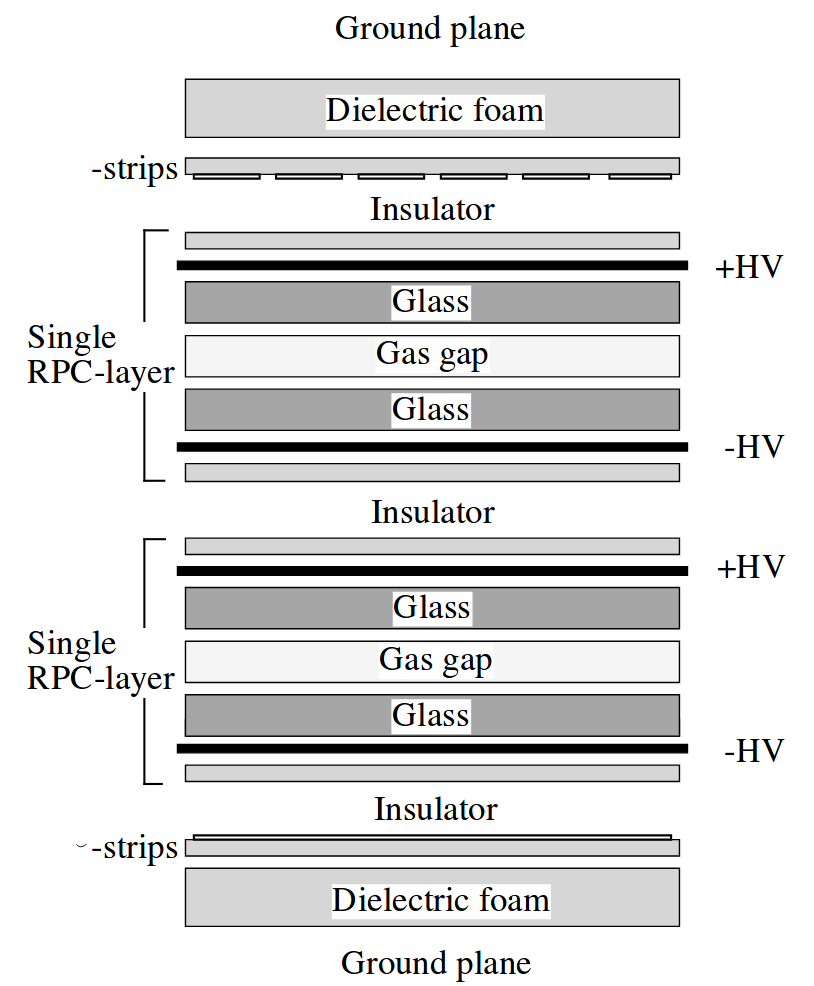
\includegraphics[width=0.4\linewidth]{fig/setup/KLM_layer}
	\caption{Cross-section of an RPC superlayer, consisting of an RPC pair \cite{ABASHIAN2002117}.}
	\label{fig:KLM_layer}
\end{figure}

The $K_L^0$ particle can be distinguished from other charged hadrons because they have no matched track in the CDC. The flight direction can also be inferred from the hit locations in the consecutive RPCs. Tracks of charged particles measured in CDC are extrapolated into KLM and clusters within $15^\circ$ of an extrapolated charged particle track are excluded from $K_L^0$ cluster candidates. On the other hand, muons with matched CDC tracks are able to reach the KLM if their momentum is larger than $0.5\e{GeV}/c$. They do not interact strongly and do not produce hadronic showers in the KLM, which serves as a handle on the muon identification. Figure \ref{fig:KLM_eff} (left) shows the number of neutral clusters per event and a Monte Carlo simulation of the predicted number of $K_L^0$ clusters per event. The average number of $K_L^0$ clusters per event is $0.5$. The agreement with the prediction gives us the confidence that the detector and our reconstruction software are performing correctly. Figure \ref{fig:KLM_eff} (right) shows the muon detection efficiency as a function of  momentum and shown for a likelihood cut of $0.66$, where muon likelihood is based on the comparison of the measured range of a particle with the predicted range for a muon. Based on $K_S \to \pi^+\pi^-$ events, a muon identification efficiency of better than $90\%$ is determined,  with a pion fake rate of less than $5\%$ for particles with momenta more than $1.5\e{GeV}/c$ and a likelihood cut of $0.66$.

\begin{figure}[H]
	\centering
	\captionsetup{width=0.8\linewidth}
	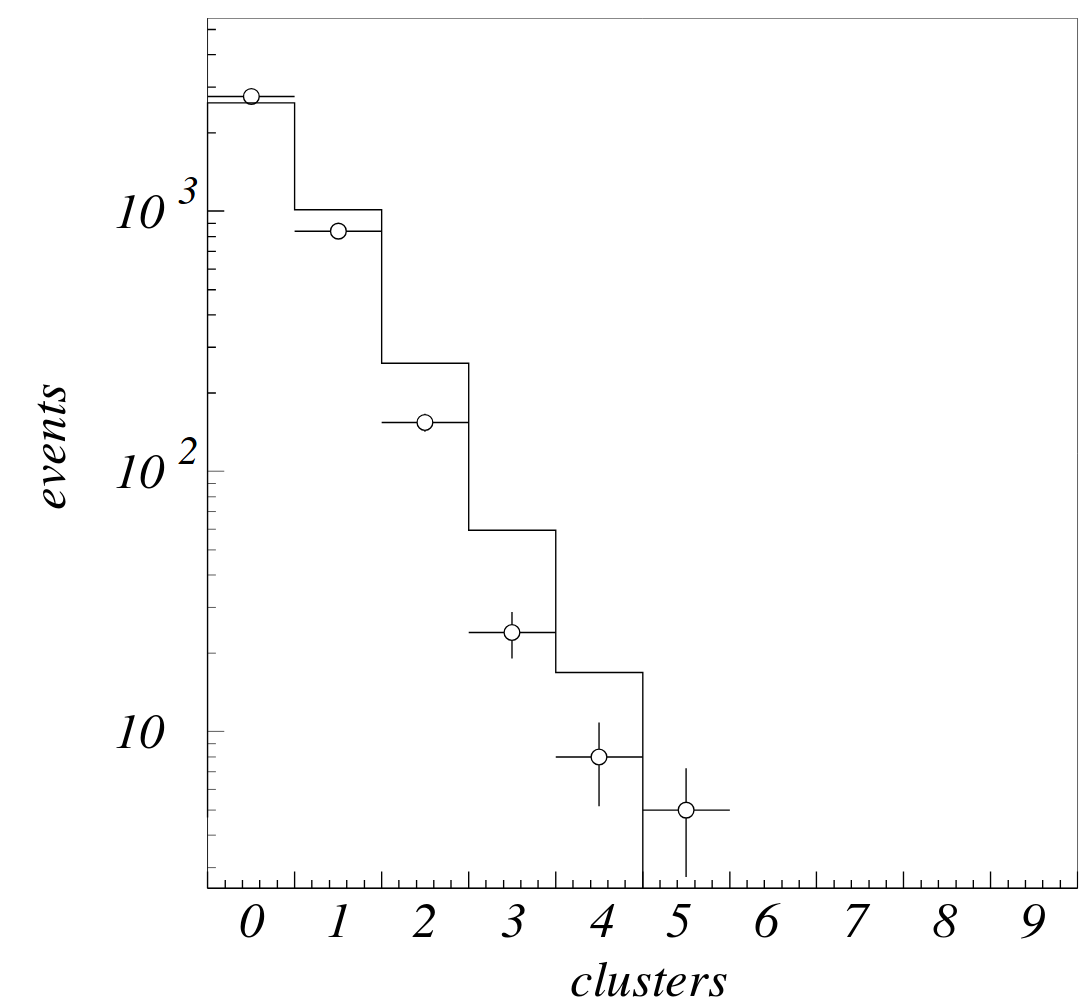
\includegraphics[width=0.48\linewidth,trim = 0cm -1.5cm 0cm 0cm]{fig/setup/KLM_clusters}
	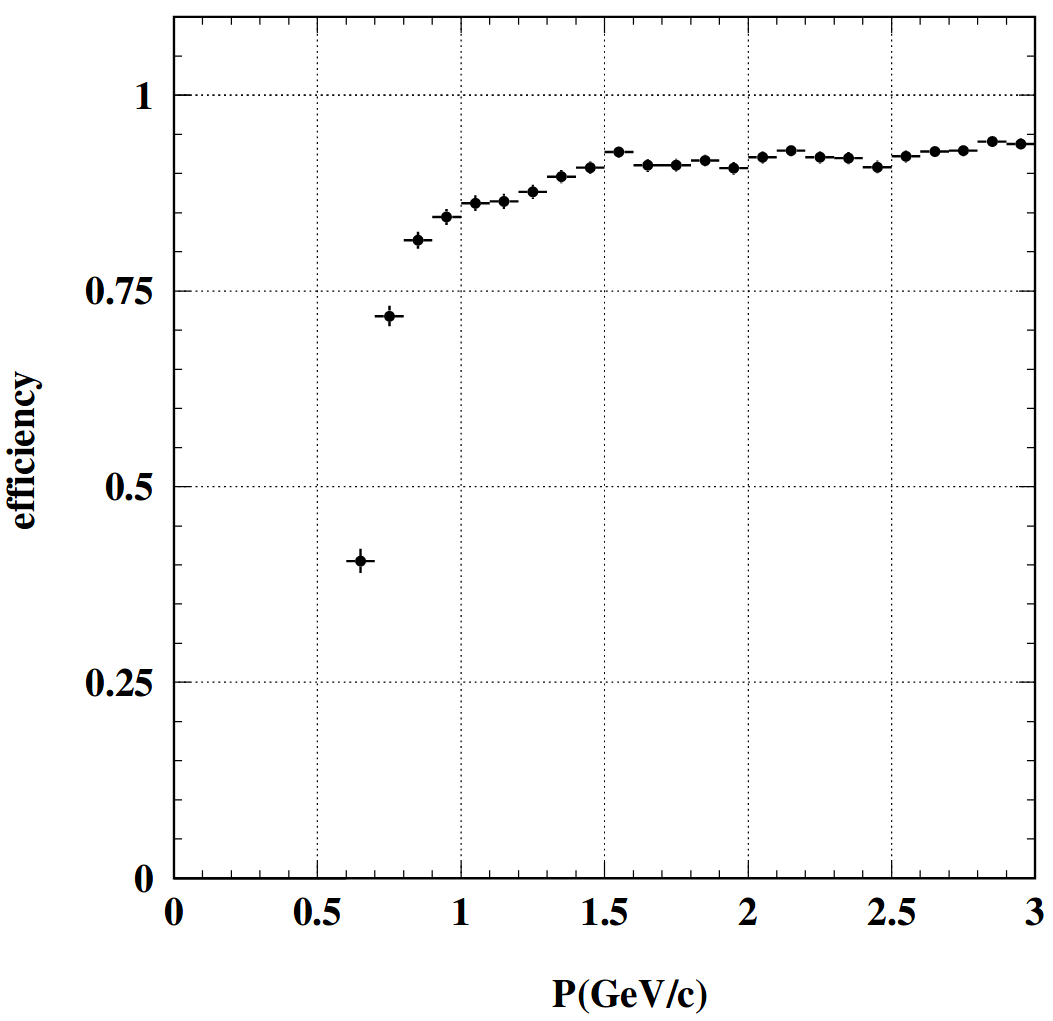
\includegraphics[width=0.48\linewidth]{fig/setup/KLM_efficiency}
	\caption{Number of neutral clusters per event in KLM (left) and muon detection efficiency as a function of momentum in KLM (right) \cite{ABASHIAN2002117}.}
	\label{fig:KLM_eff}
\end{figure}

Cosmic ray events have been used to determine efficiency and resolution of the KLM, with an overall efficiency typically over $98\%$. The temporal and spatial resolution of the KLM are few$\e{ns}$ and about $1.2\e{cm}$, respectively. The latter corresponds to an angular resolution from the interaction point of better than $10\e{mrad}$.

In order to to detector calibration and proper luminosity measurements, we need to accumulate samples of Bhabha and $\gamma\gamma$ scattering. Otherwise, as shown in Table \ref{tab:xsec}, the cross-section for physics events of interest is reasonably small. During normal operation (luminosity of $L = 10\E{34}\e{cm^{-2}s^{-1}}$) the total event rate is around $200\e{Hz}$, which is well below the data acquisition (DAQ) limit of $500\e{Hz}$. Out of this rate, $100\e{Hz}$ are physically interesting events, which include also two photon events, Bhabha scattering and $\mu$ pair production, besides hadronic events from $B \bar B$ pair events. In order to discard events which are not interesting for physics analyses, we use a trigger system by appropriately applying restrictive conditions. This section describes the necessary procedures and equipment to successfully do so.

\subsubsection{Trigger System}
The trigger system operates by immediately eliminating events that are not of interest, so that the amount of stored data is within the $500\e{Hz}$ frequency limit, while the efficiency for physics events of interest is kept high. Events which pass the triggers are then stored, otherwise discarded. The Belle trigger system consists of three stages, Level-1 (L1) online hardware trigger, Level-3 (L3) online software trigger and Level-4 (L4) offline software trigger.

L1 trigger is the first stage of the trigger system, which consists of multiple sub-detector triggers, all connected to a central trigger system called the Global Decision Logic (GDL), as schematically shown in Figure \ref{fig:TRG_GDL}. Each sub-detector trigger works on a principle of either a track trigger or an energy trigger. In the former case the triggers discard events not meeting conditions based on the number of reconstructed tracks or track hits, while the latter is based on the total energy deposit and counting of crystal hits. Each sub-detector processes the event information and provides it to the GDL, where all the information is combined and the current event is characterized. The information from the sub-detector triggers reaches the GLD within $1.85\e{\mu s}$ after the collision, and the final trigger signal is provided within at a fixed $2.2\e{\mu s}$ latency. The combined efficiency from the L1 trigger is greater than $99.5\%$ for hadronic events.

\begin{figure}[H]
	\centering
	\captionsetup{width=0.8\linewidth}
	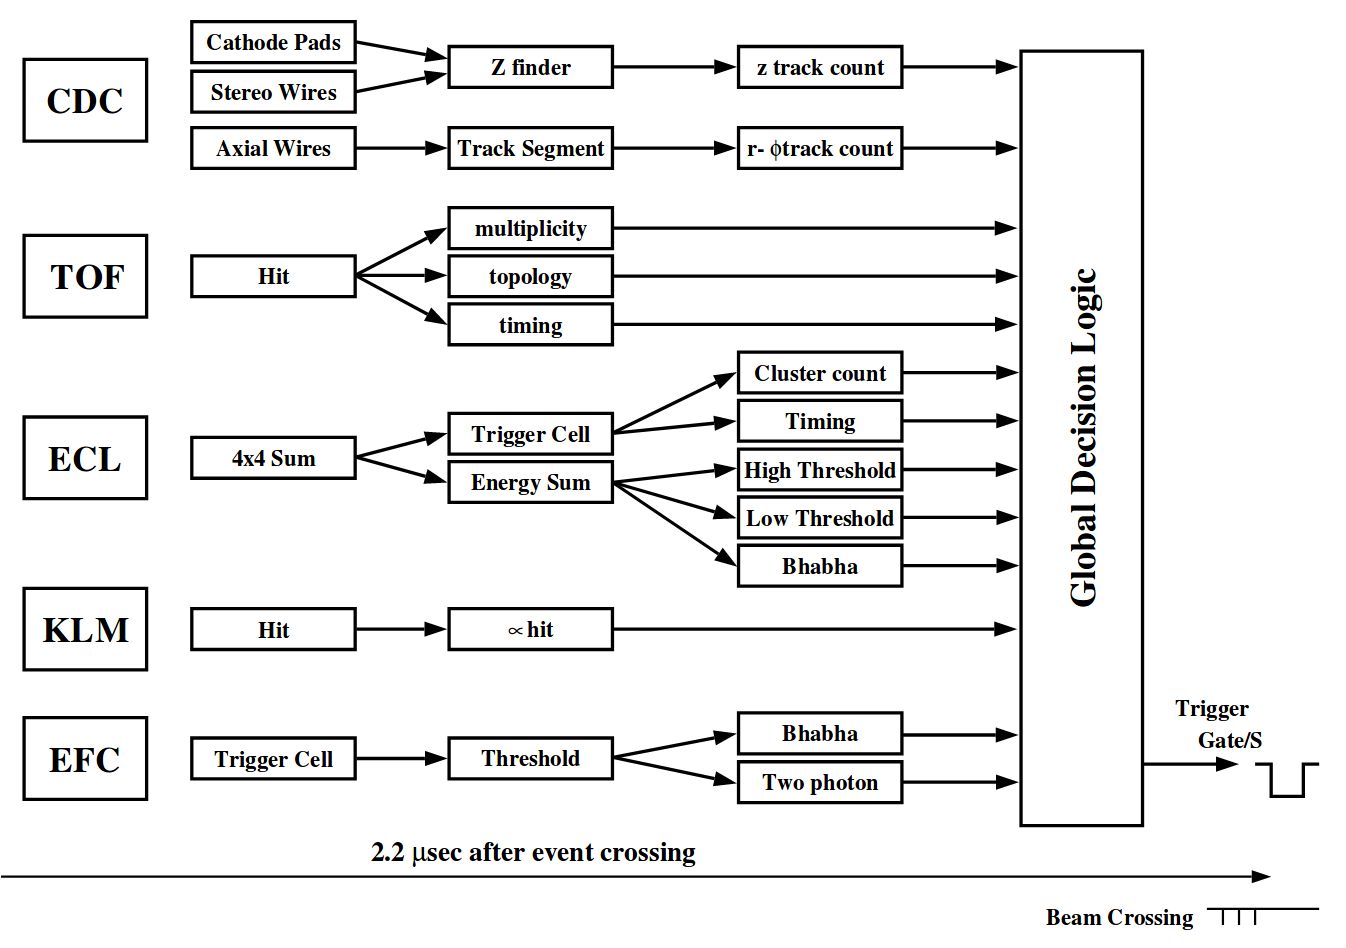
\includegraphics[width=0.8\linewidth]{fig/setup/TRG_GDL}
	\caption{The Level-1 trigger system for the Belle detector \cite{ABASHIAN2002117}.}
	\label{fig:TRG_GDL}
\end{figure}

After passing L1 trigger, the L3 discards background events from the software-wise perspective. L3 is an online software trigger which performs a simple, but fast reconstruction of the event. Events with at least one track satisfying the impact parameter condition $\vert\mathrm{d}z \vert < 5.0\e{cm}$ and with a total energy deposit in the ECL more than $1\e{GeV}/c$ are selected. The L3 trigger reduces the event rate by $50\%$, with a $99\%$ efficiency for hadronic events.

After passing the L3 trigger, the events are recorded on tapes. However, these data still contain many events from the beam background. To reduce the background events even further, they are required to pass the L4 offline software filtering. At the same time, high efficiencies for signal events is still required. Events must satisfy the following conditions
\begin{itemize}
	\item have at least one track with $p_T > 300\e{MeV}/c$ and impact parameters $\vert \mathrm{d}r \vert < 1.0\e{cm}$ and $\vert \mathrm{d}z \vert < 4.0\e{cm}$,
	\item have total energy deposit in the ECL must greater than $4\e{GeV}$.
\end{itemize}
Approximately $27\%$ of triggered events are passed through L4, while keeping an almost full efficiency for hadronic events. Events that pass the L4 trigger are fully reconstructed and stored to the DST. Overall, the efficiency of hadronic events after all trigger stages is measured to be more than $99\%$, which is more than the requirements from physics analyses.

\section{Postopek analize}
\section{Sistematske negotovosti}
\section{Kon\v cni rezultat}

\end{otherlanguage}
\end{document}


